\section{Результаты}

\begin{frame}
\frametitle{Интерфейс системы}
\begin{figure}
    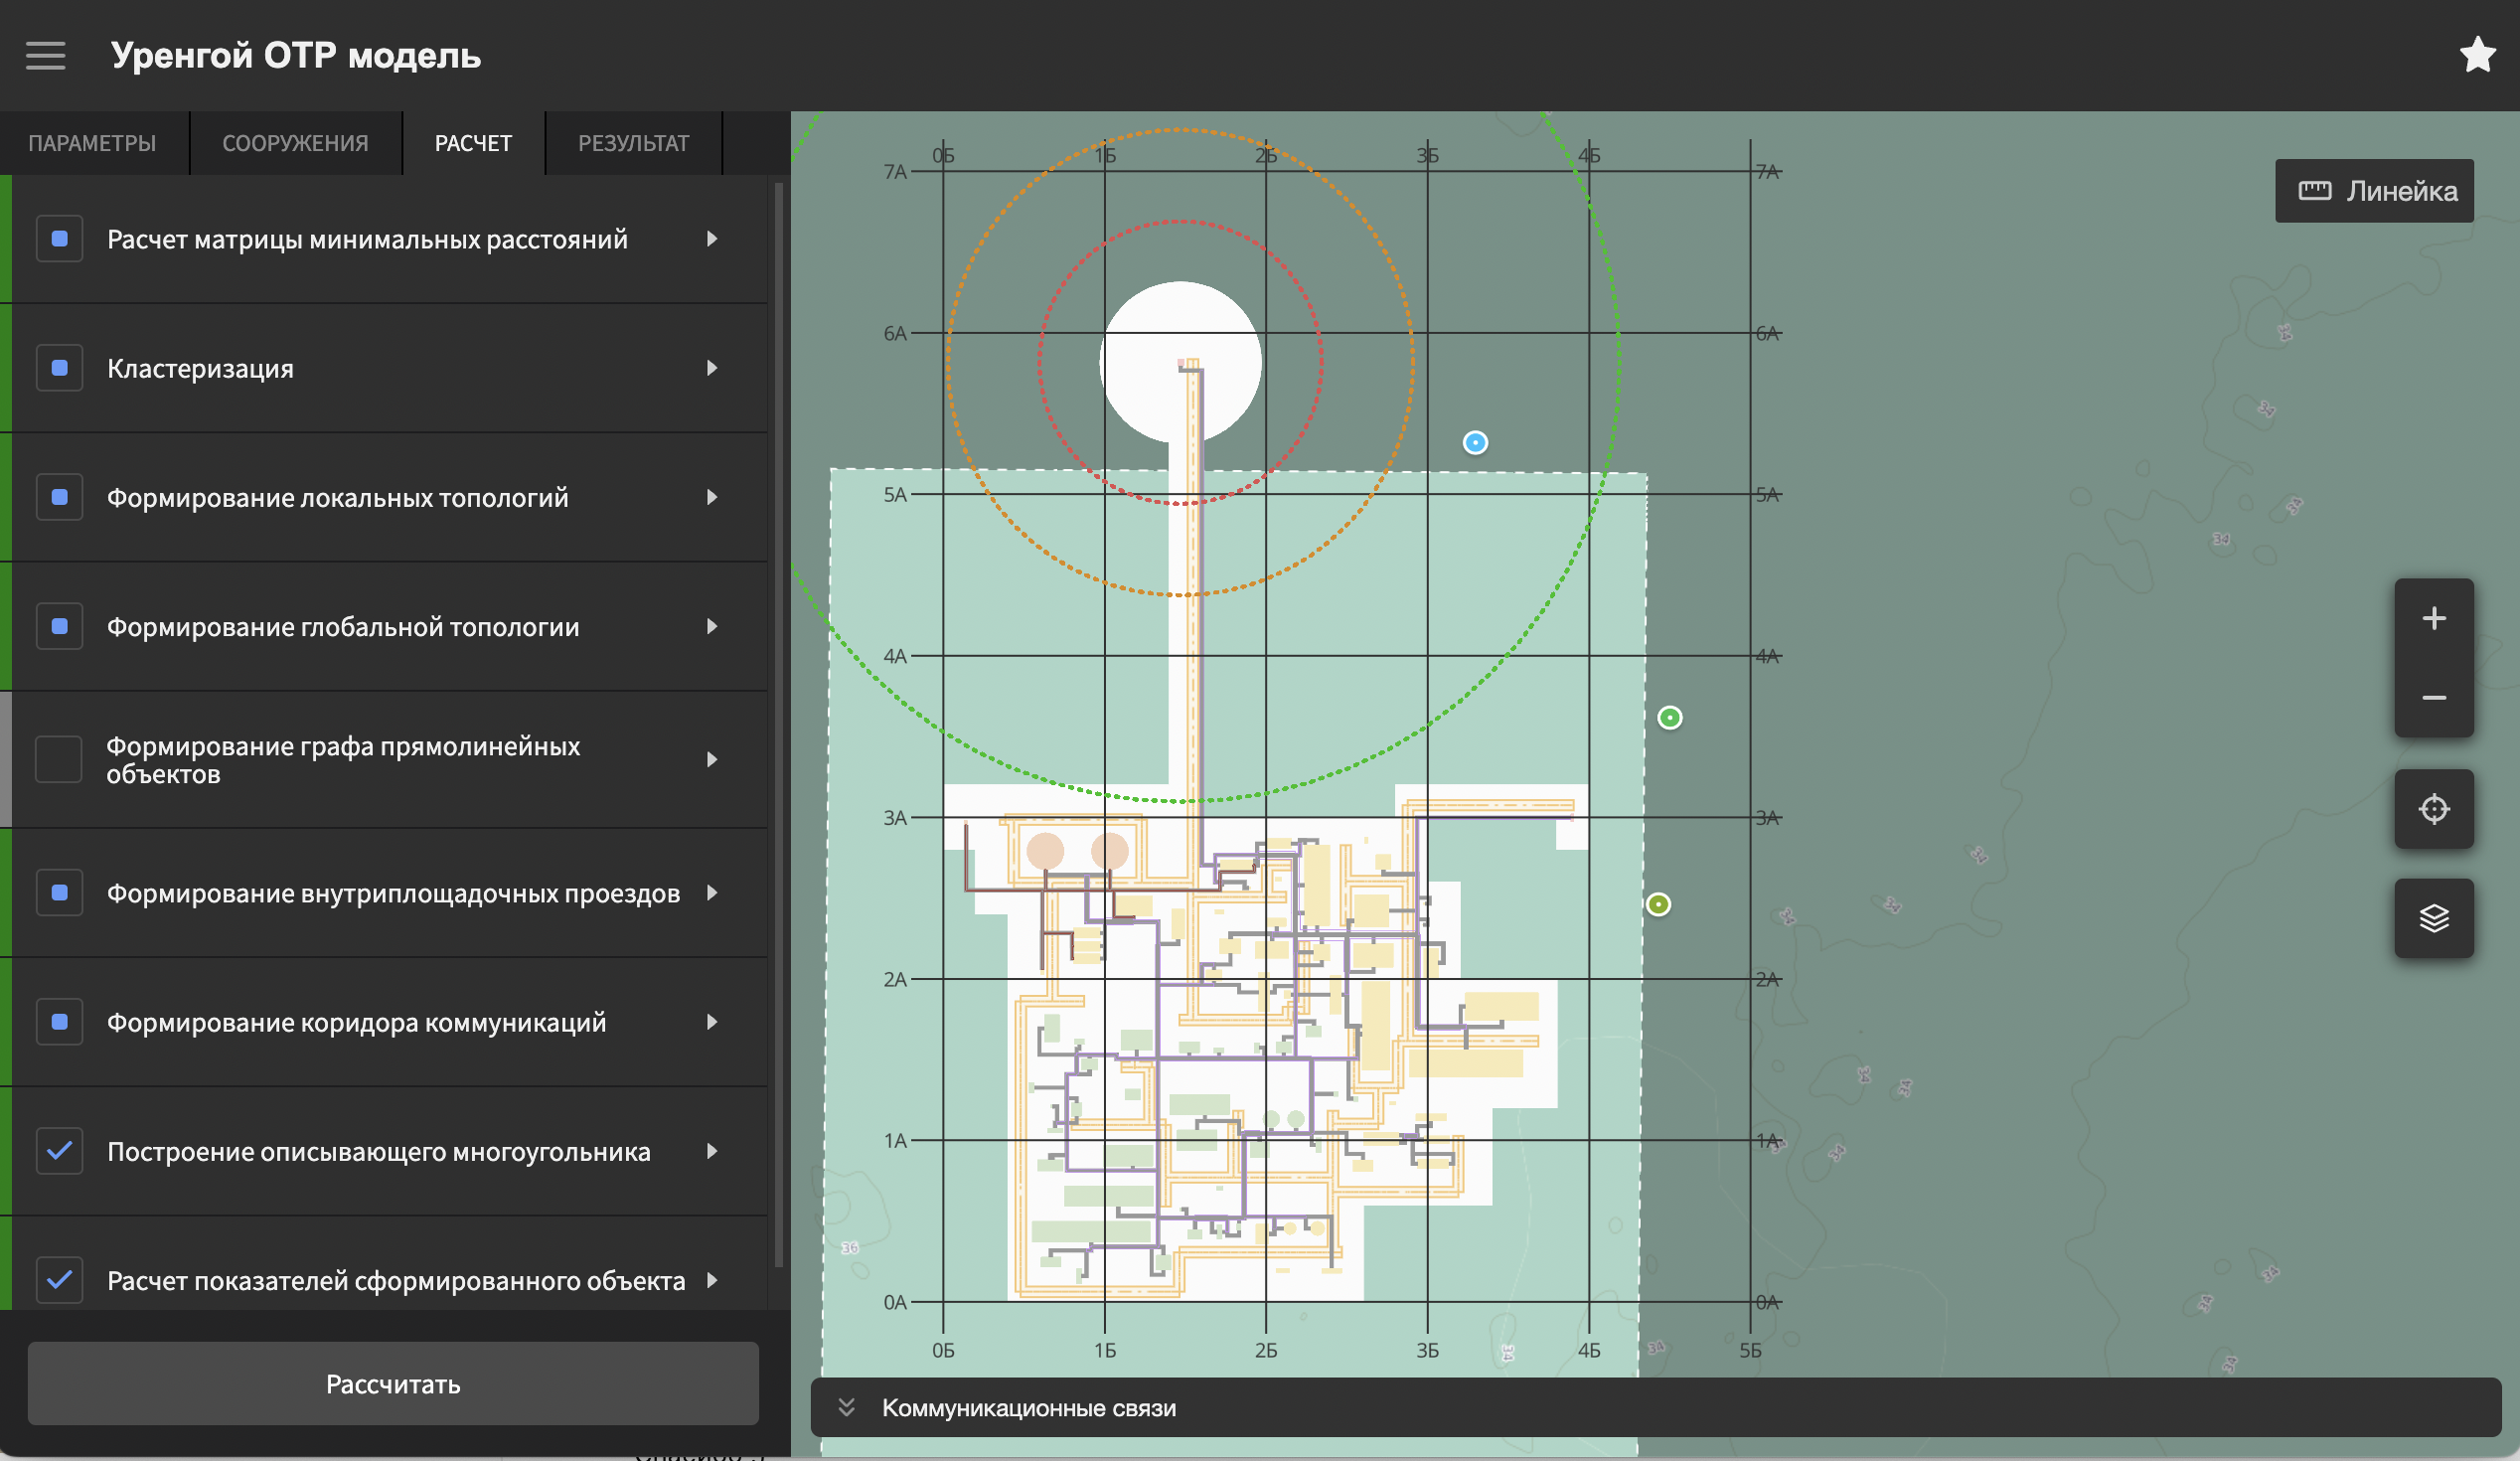
\includegraphics[scale=0.1391]{pictures/results/plan-system}
\end{figure}
\end{frame}


\begin{frame}
\frametitle{Результаты}
\begin{itemize}
    \item собраны и проанализированы требования пользователей;
    \item сформированы функциональные и нефункциональные требования к программному компоненту;
    \item cпроектирована системная и программная архитектура расчётного модуля;
    \item {
           реализован расчётный модуль, состоящий из пяти программных компонент:
            \begin{enumerate}
                \item математическая библиотека,
                \item расчётная модель данных,
                \item сервис запуска расчётных задач,
                \item сервис хранения расчётных данных,
                \item сервис запуска математических методов.
            \end{enumerate}
    }
\end{itemize}
\end{frame}

